\subsection{Salidas históricas de un paso}

\begin{figure}[htbp]
\centering
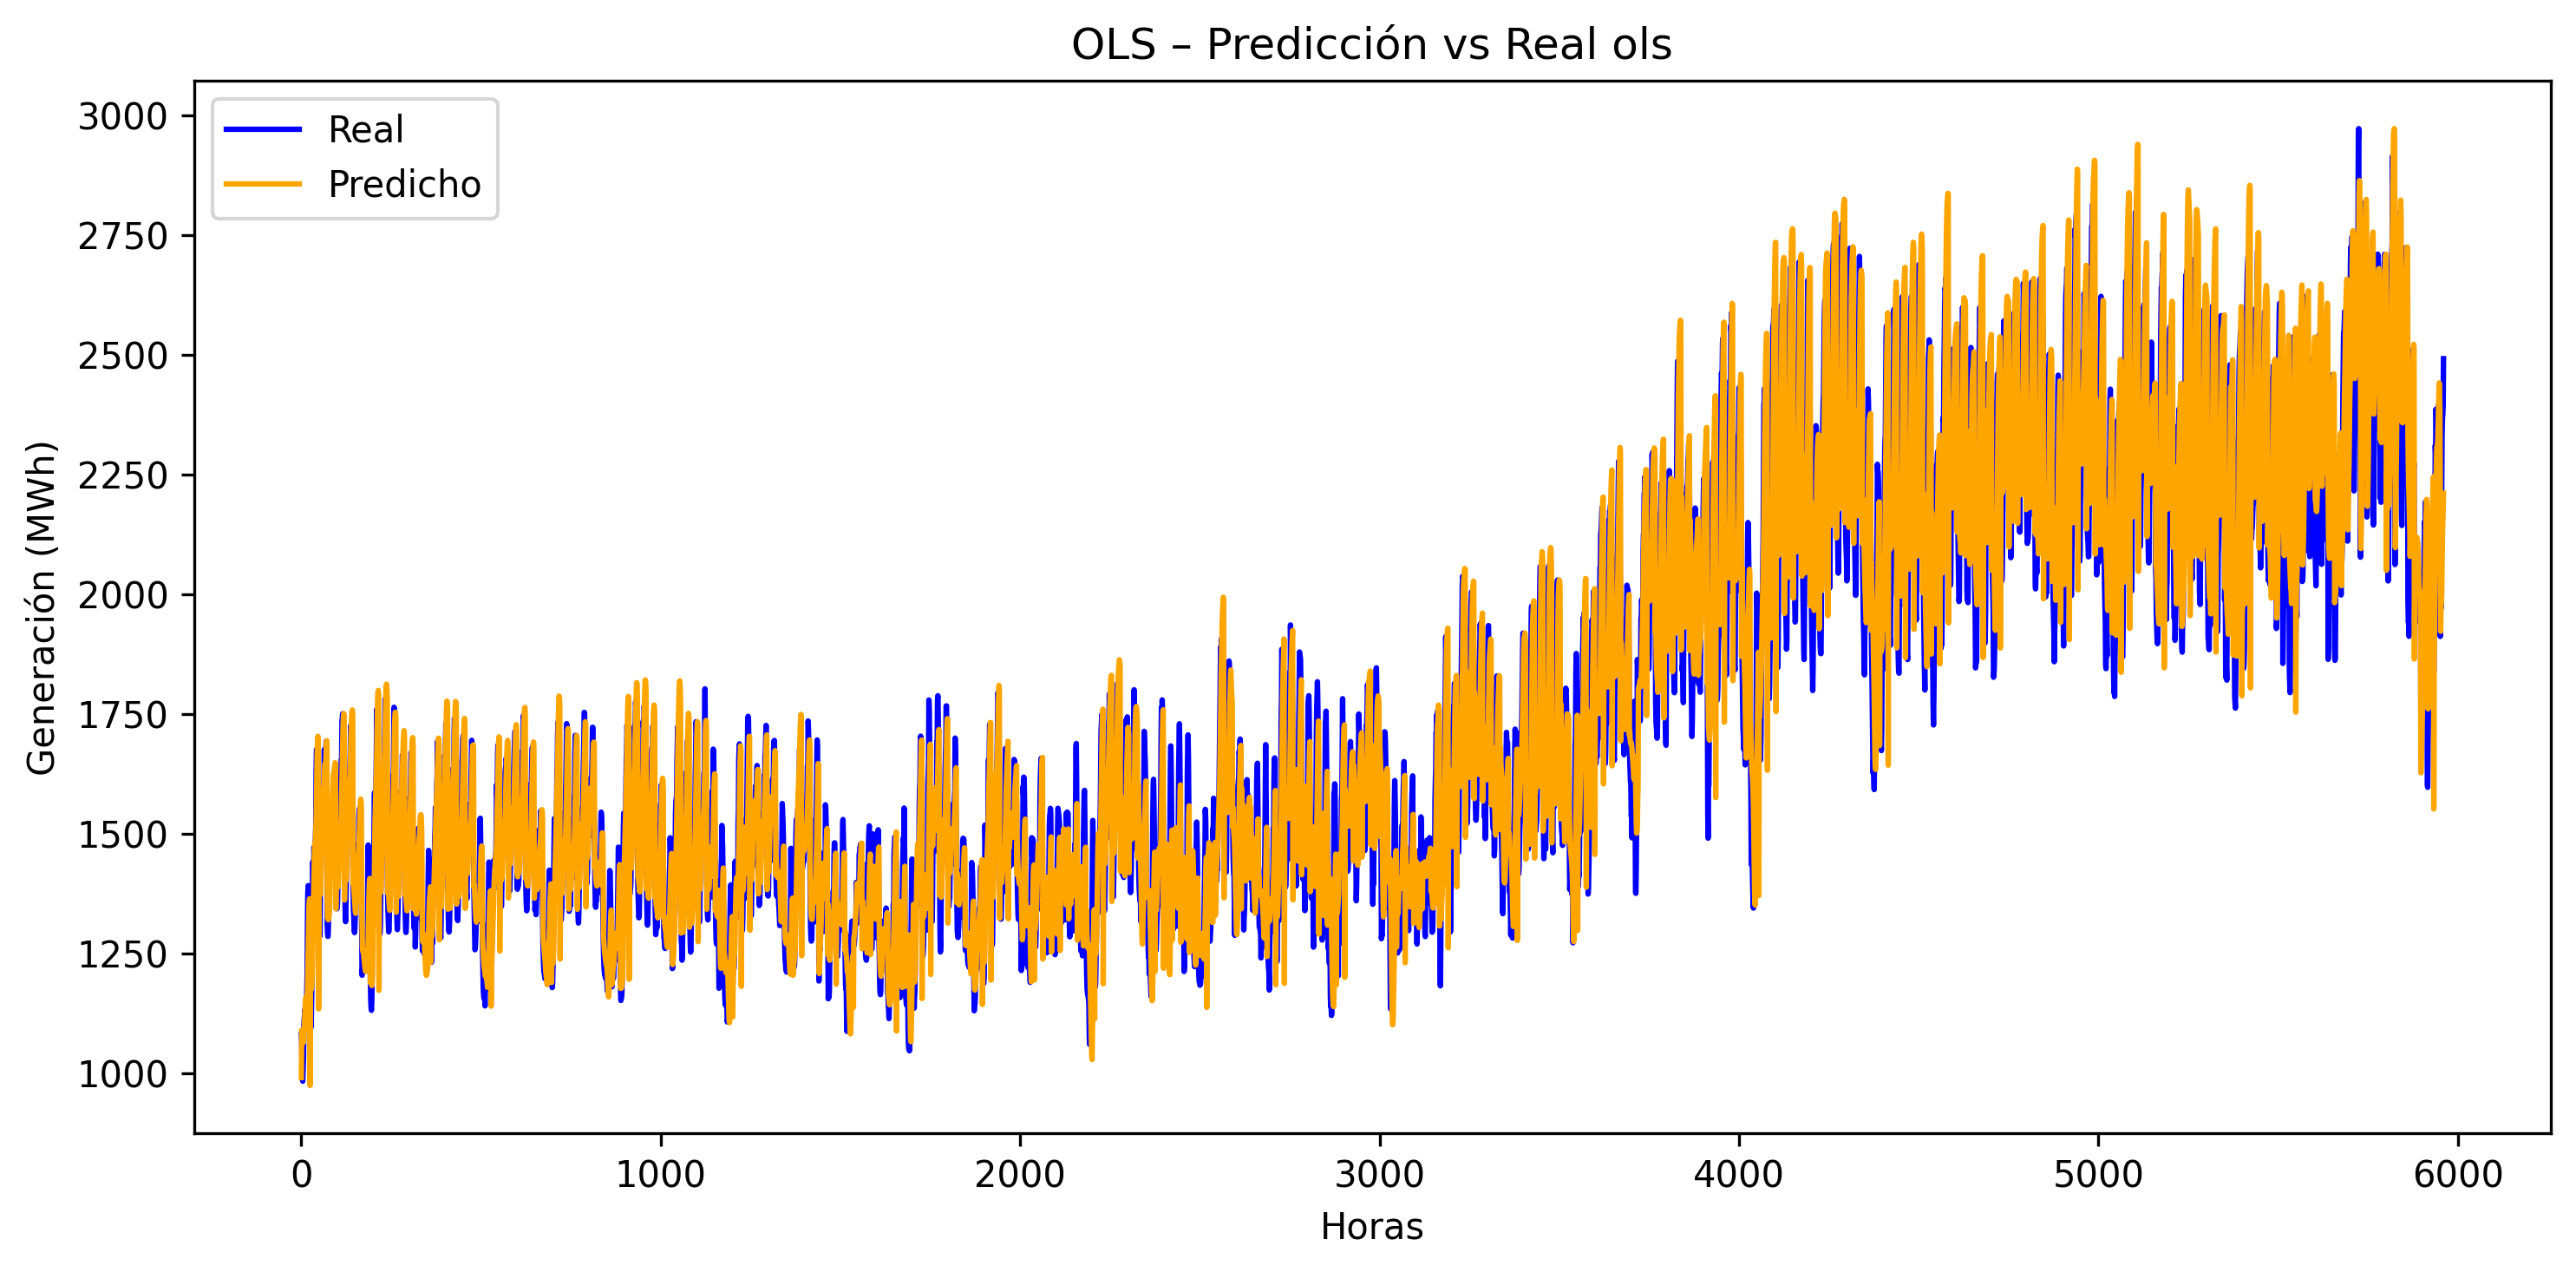
\includegraphics[width=\textwidth]{figuras/05_resultados/ols_calendario_historico.png}
\caption{Salida histórica de OLS con predictores de calendario para la comparación entre generación observada y estimada. El eje horizontal representa la secuencia de predicciones.}
\label{fig:ols-un-paso}
\end{figure}

En la figura~\ref{fig:ols-un-paso}, la trayectoria estimada reproduce visualmente las oscilaciones generales y el aumento de nivel hacia la parte final de la secuencia. Se observan diferencias locales en máximos y mínimos. La superposición de trazos permite examinar el seguimiento global, pero no establece por sí sola la magnitud del error ni la ausencia de sesgo.

\begin{figure}[htbp]
\centering
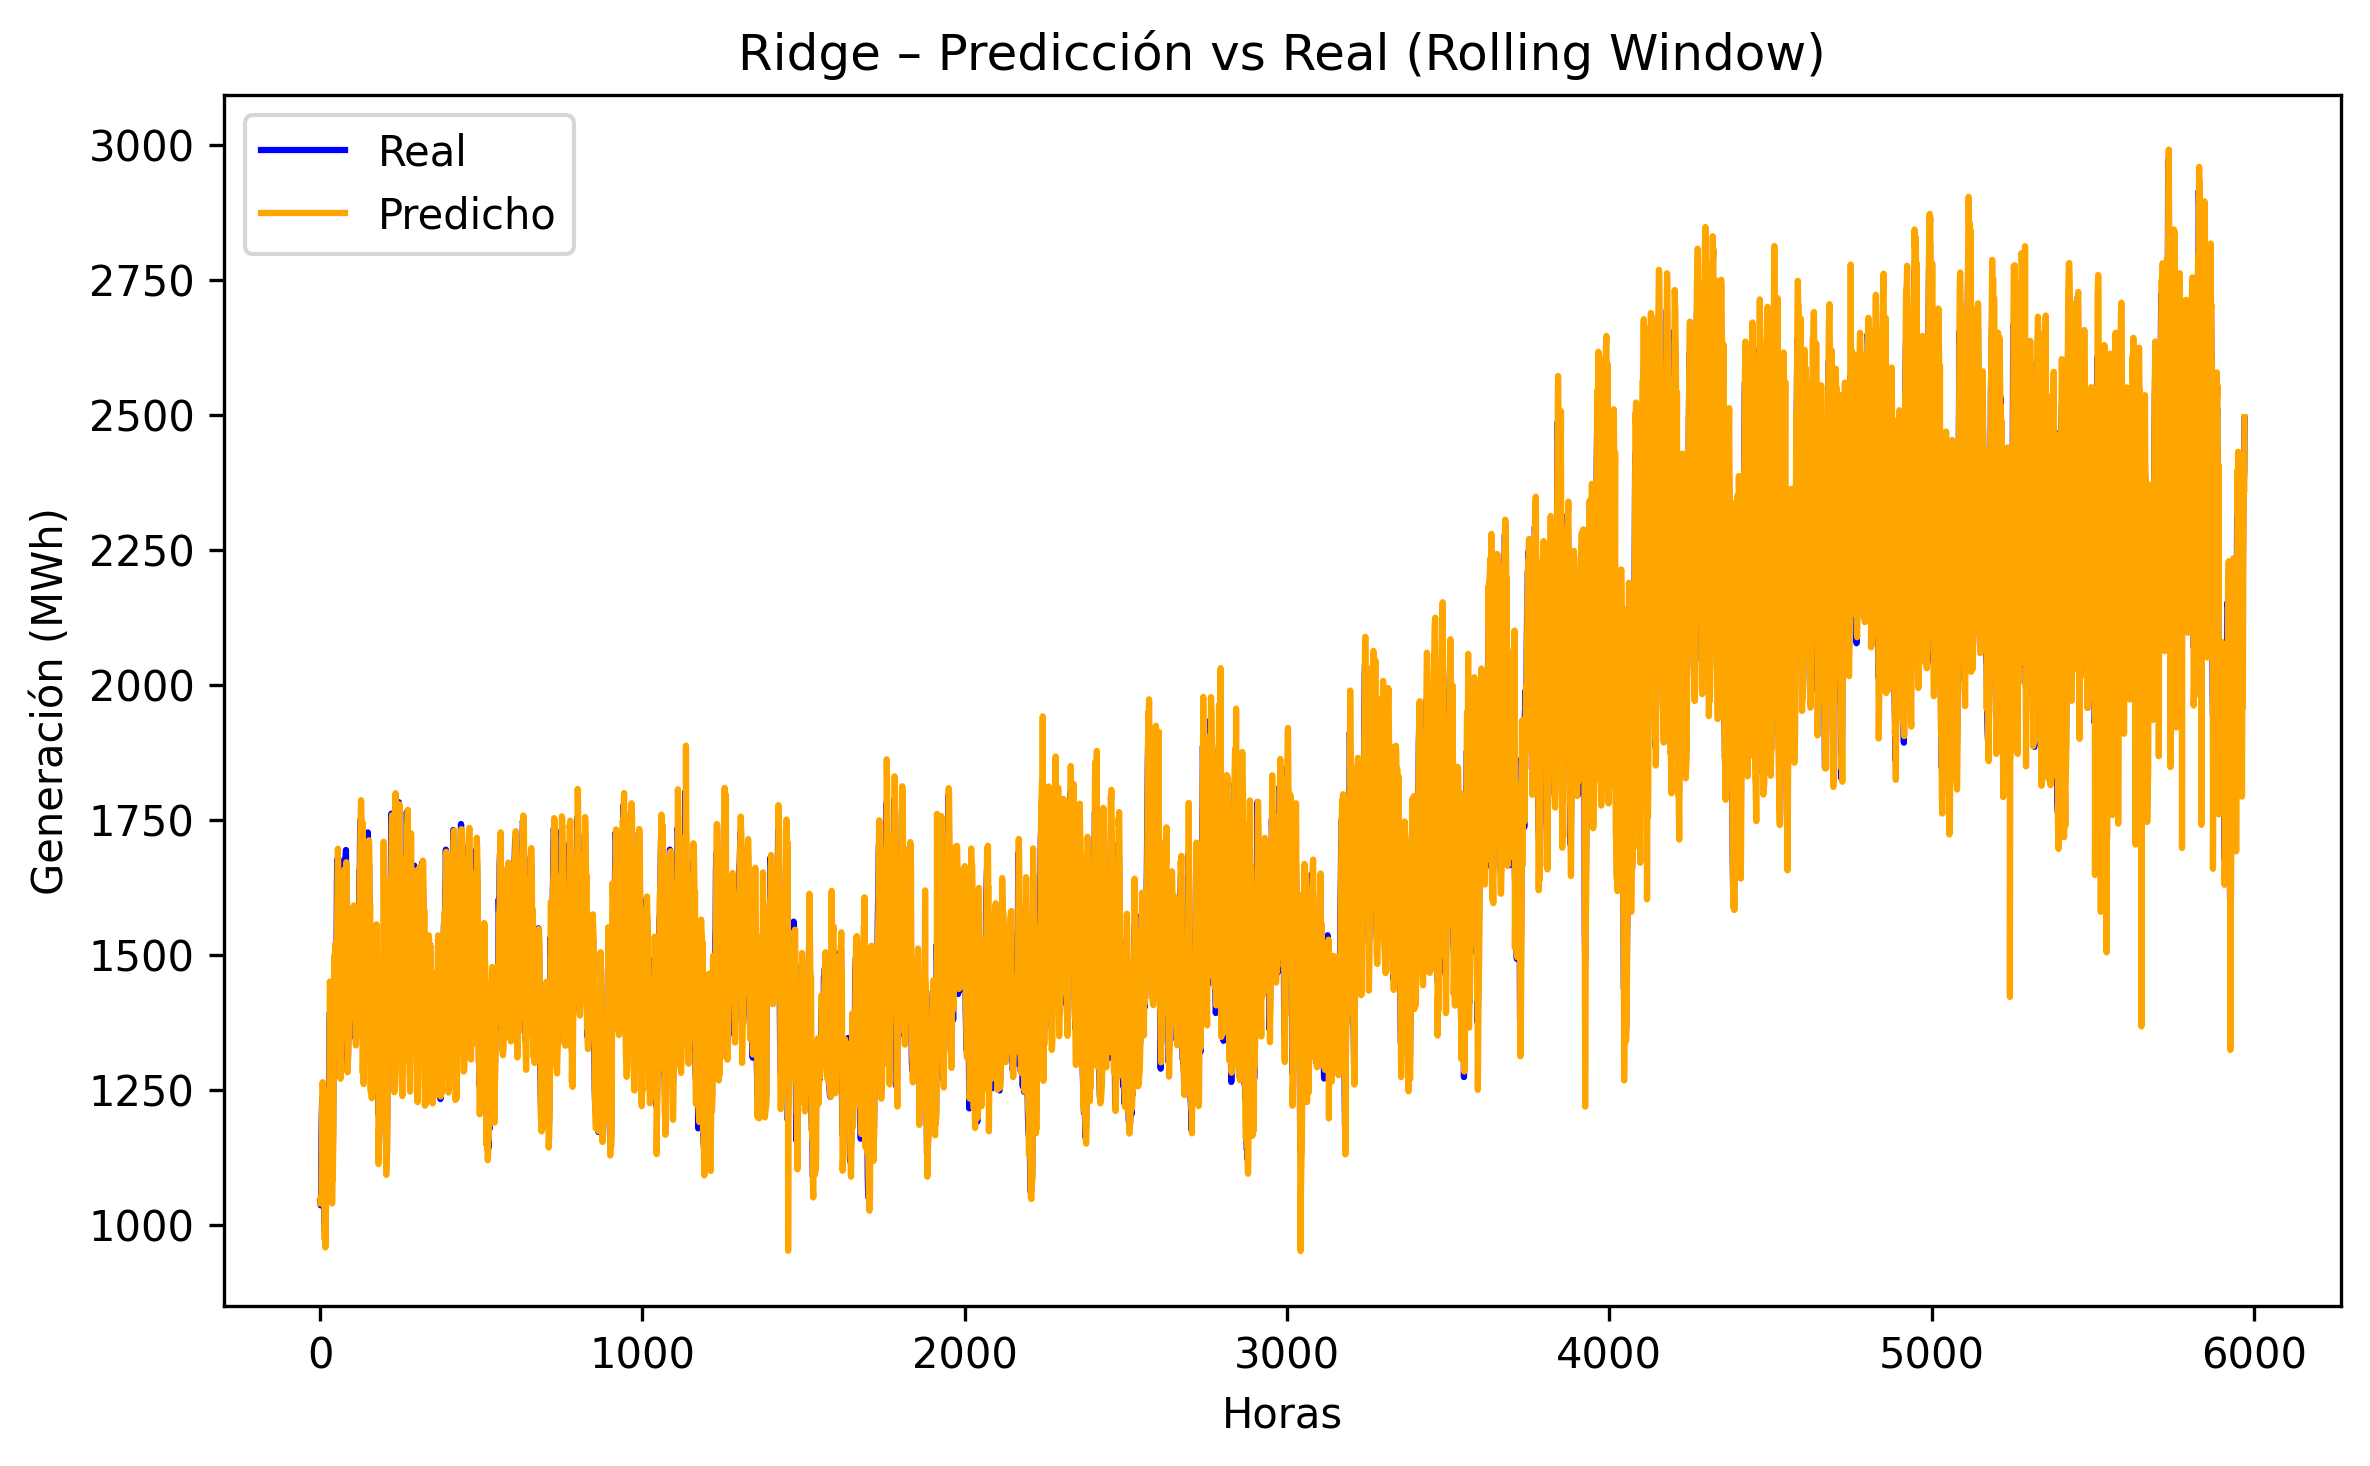
\includegraphics[width=\textwidth]{figuras/05_resultados/ridge_un_paso.png}
\caption{Salida conservada de Ridge con ventana móvil. La alta superposición de curvas limita la identificación visual de errores puntuales.}
\label{fig:ridge-un-paso}
\end{figure}

La figura~\ref{fig:ridge-un-paso} presenta una superposición amplia entre valores observados y estimados, tanto en el tramo de menor generación como en el de mayor nivel. Este comportamiento es compatible con un seguimiento cercano de la serie representada, aunque no permite concluir que Ridge supera a OLS. Además de no contar con métricas verificables para estas imágenes, los programas difieren en entradas, longitud de historia y escalamiento.
